\documentclass[tikz, dvipdfmx]{standalone}
\usepackage{tikz}
\usepackage{bm}
\usepackage{tikz-feynhand}

\usetikzlibrary{intersections,calc,arrows.meta}
\begin{document}
  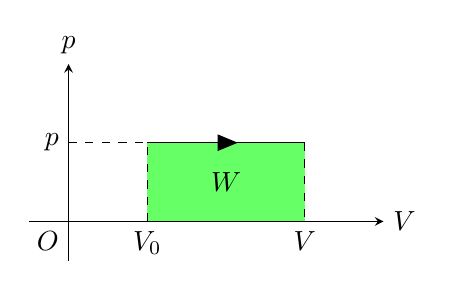
\begin{tikzpicture}
    \coordinate[label=below left:$O$] (O) at (0,0);
    \coordinate (A) at (1,1);
    \coordinate (B) at (3,1);
    \coordinate (XS) at (-0.5,0);
    \coordinate (XL) at (4,0);
    \coordinate (YS) at (0,-0.5);
    \coordinate (YL) at (0,2);
    \coordinate[label=left:$p$] (P) at($(YS)!(A)!(YL)$);
    \coordinate[label=below:$V_0$] (V0) at($(XS)!(A)!(XL)$);
    \coordinate[label=below:$V$] (V) at($(XS)!(B)!(XL)$);

    \draw [->, >=stealth] (XS) -- (XL) node[right]{$V$};
    \draw [->, >=stealth] (YS) -- (YL) node[above]{$p$};
    \fill[green, opacity=0.6] (A) rectangle (V);
    \begin{feynhand}
    \propag[fer] (A) to (B);
    \end{feynhand}
    \draw[dashed] (P) -- (A) -- (V0);
    \draw[dashed] (B) -- (V);
    \draw (2,0.5) node{$W$};
  \end{tikzpicture}
\end{document}
